\chapter*{Descrizione generale}

\section*{Introduzione}
L'applicazione WORTH fornisce quasi tutti i servizi tramite interazione \textbf{Client-Server} fatta esclusione della chat di progetto che lavora in modalità \textbf{Peer-to-Peer}.
\section*{Tipi di connessione utilizzati}
\begin{center}
\end{center}
\subsection*{Java RMI}
Tramite una funzione \code{register(username, hash)} il client\\ richiede la registrazione di un nuovo utente al servizio.
\subsection*{Java RMI Callback}
Il server fornisce al client la lista degli utenti registrati e notifica i cambiamenti di stato \code{(online - offline)}.
\subsection*{UDP Multicast}
Ogni progetto ha associata una chat tramite la quale i membri possono comunicare, l'indirizzo di questa chat viene fornito dal server tramite la connessione TCP ma i messaggi vengono poi trasferiti direttamente da un client agli altri.
\subsection*{TCP}
Tramite una connessione TCP persistente (creata al momento della richiesta di accesso al servizio) un client puo' effettuare delle operazioni sui dati sui quali ha accesso sul server come:creazione di un progetto, aggiunta di un membro, movimento di una card\dots
\newline
I comandi TCP sono codificati come descritto all'interno del file 
\begin{center}
    \code{worth/common/CMD.java}
\end{center}
Un esempio di comando e':
\code{{\color{blue}0x10}<username>{\color{red}0x03}<hash>{\color{red}0x03}}
\begin{description}
    \item[\code{\color{blue}0x10}] Codice identificativo del comando di login.
    \item[\code{<username>}] Nome utente codificato come sequenza di byte
    \item[\code{\color{red}0x03}] Identifica la fine di un parametro.
    \item[\code{<hash>}] hash della password codificato come sequenza di byte
\end{description}
\section*{Scelte d'implementazione}
\paragraph*{Interfaccia} L'utente finale interagisce con il server tramite un'interfaccia grafica sviluppata tramite la piattaforma JavaFX.
\paragraph*{Persistenza dei file di progetto} Ogni volta che viene fatta una modifica ad un progetto viene ricreato e scritto su file-system un file json contenente il nome del progetto, le card associate, e i membri di esso.
\paragraph*{Persistenza dei file delle card} Ogni volta che viene fatta una modifica ad una card virene ricreato e scritto su file-system un file json contenente il nome della card, la descrizione, e lo storico di tutti i suoi movimenti.
\paragraph*{Identificazione utenti} Per non spedire e memorizzare le password in chiaro, il client, in fase di registrazione e di login, la trasforma in un hash.
\paragraph*{Persistenza degli utenti registrati} Gli usernames e gli hash associati sono salvati sul file-system come una sequenza di valori
\begin{center}
    \code{<username>:<hash>}
\end{center}
E' stato scelto di non utilizzate un file JSON per questo parametro perché altrimenti all'aggiunta di un nuovo utente sarebbe stato necessario riscrivere l'intero file da capo.

\chapter*{Threads e controllo di concorrenza}
\section*{Lato server}
Il server, al momento, non attiva alcun thread supplementare rispetto al main dato che gestisce le connessioni TCP tramite multiplexing dei canali con NIO.
La classe che si occupa del multiplexing pero' e' stata implementata in modo da poter essere attivata come nuovo thread permettendo di eseguire altre operazioni sul thread main.

Per gestire la concorrenza tutte le strutture dati principali utilizzano classi thread safe come la \code{ConcurrentHashMap}
\section*{Lato client}
Il client attiva un thread per la gestione della GUI e, al momento dell'apertu\-ra di una chat, un thread che si occupa della ricezione e dell'invio dei messaggi sul gruppo multicast.

\chapter*{Descrizione delle classi}

La struttura del progetto e' divisa in 3 packages principali:
\begin{description}
    \item[client] Contiene tutte le classi utilizzate per il funzionamento del client.
    \item[server] Contiene tutte le classi utilizzate per il funzionamento del server.
    \item[common] Contiene le interfacce per la comunicazione RMI e le strutture dati che devono restare immutate tra client e server.
\end{description}
\section*{client}

\dirtree{%
.1 client.
.2 chat.
.3 Chat.java.
.2 gui.
.3 Card.java.
.3 GUI.java.
.3 LoginController.java.
.3 MenuController.java.
.3 login.fxml.
.3 menu.fxml.
.2 tcp.
.3 Commands.java.
.3 Connection.java.
.3 Response.java.
.2 users.
.3 Callback.java.
.3 Users.java.
.2 utils.
.3 Arguments.java.
.3 Const.java.
.3 NoSelectionModel.java.
.3 Utils.java.
.2 clientMain.java.
}

\begin{description}
    \item[clientMain.java] {\color{red}Main class}
    \item[chat] si occupa della ricezione e dell'invio dei messaggi nel giusto gruppo multicast.
    \item[gui] Le classi all'interno di questo package si occupano di mostrare l'interfac\-cia grafica all'utente e di gestire le richieste provenienti da essa.
    \item[tcp] Contiene le classi di supporto alla comunicazione TCP per l'invio delle richieste al server.
    \item[users] Package che si occupa di mantenere le liste degli utenti e il loro stato, e aggiornarle tramite RMI callback.
    \item[utils] Contiene tutte le classi di supporto.
\end{description}

\section*{server}
\dirtree{%
.1 server.
.2 projects.
.3 Card.java.
.3 Projects.java.
.3 Project.java.
.2 tcp.
.3 Connection.java.
.2 users.
.3 Users.java.
.3 User.java.
.3 RegisterService.java.
.3 Callback.java.
.2 chat.
.3 IPGen.java.
.2 utils.
.3 Utils.java.
.3 Arguments.java.
.3 ConcurrentHashSet.java.
.3 Const.java.
.2 mainServer.java.
}

\begin{description}
    \item[mainServer.java] {\color{red}Main class}
    \item[projects] Contiene le classi utili alla creazione e modifica di tutti i dati dei progetti.
    \item[tcp] Contiene la classe \code{Connection.java}, utilizzata per l'apertura della socket per l'accettazione delle richieste TCP e per l'interpretazione dei comandi in arrivo.
    \item[users] Contiene il \textit{database} degli utenti registrati e tutte le operazioni per essi, oltre alle classi utilizzate per la notifica degli utenti al client tramite callback.
    \item[chat] La classe \code{IPGen.java} e' utilizzata per la creazione di indirizzi multicast unici per ogni progetto.
    \item[utils] Contiene tutte le classi di supporto.
\end{description}

\section*{common}

\dirtree{%
.1 common.
.2 CMD.java.
.2 Status.java.
.2 CallbackInterface.java.
.2 CallbackServerInterface.java.
.2 RegisterServiceInterface.java.
}

\begin{description}
    \item[CMD.java] Contiene la descrizione e il codice dei comandi utilizzabili sulla connessione TCP.
    \item[Status.java] Enum usato per distinguere gli stati in cui possono trovarsi le card.
    \item[*Interface.java] Interfacce per la definizione dei metodi usati da RMI. 
\end{description}

\chapter*{Guida all'utilizzo}

Per utilizzare WORTH e' necessario installare Java 8 o superiore

\section*{Server}

\subsection*{Librerie utilizzate}
\begin{itemize}
    \item \href{http://search.maven.org/remotecontent?filepath=com/github/jankroken/commandline/1.7.0/commandline-1.7.0.jar}{CommandLine} Utilizzata per il parsing dei comandi su riga di comando. (\href{https://github.com/jankroken/commandline}{source})
    \item \href{https://storage.googleapis.com/google-code-archive-downloads/v2/code.google.com/json-simple/json-simple-1.1.1.jar}{JSONSimple} Utilizzata per convertire oggetti in stringhe JSON. (\href{https://github.com/fangyidong/json-simple}{source})
\end{itemize}
Tutte le librerie sono gia presenti nella cartella \code{lib}
\subsection*{Esecuzione}
Per far partire il server basta eseguire lo script \code{server.sh}.
E' permessa la modifica di alcuni parametri tramite argomenti da riga di comando, per conoscerli basta eseguire
\begin{center}
    \code{server.sh -h}
\end{center}
\subsection*{Salvataggio dati}
I dati persistenti sono salvati all'interno della cartella \code{files}

\section*{Client}

\subsection*{Librerie utilizzate}
\begin{itemize}
    \item \href{http://search.maven.org/remotecontent?filepath=com/github/jankroken/commandline/1.7.0/commandline-1.7.0.jar}{CommandLine} Utilizzata per il parsing dei comandi su riga di comando. (\href{https://github.com/jankroken/commandline}{source})
    \item \href{https://gluonhq.com/download/javafx-11-0-2-sdk-linux/}{JavaFX} Utilizzata per la creazione della GUI. (\href{https://gluonhq.com/download/javafx-11-0-2-sdk-windows/}{Windows download})
\end{itemize}
Tutte le librerie sono gia presenti nella cartella \code{lib}
\subsection*{Esecuzione}
Per far partire il client basta eseguire lo script \code{client.sh}.
E' permessa la modifica di alcuni parametri tramite argomenti da riga di comando, per conoscerli basta eseguire
\begin{center}
    \code{client.sh -h}
\end{center}
\subsection*{Utilizzo}
\begin{center}
    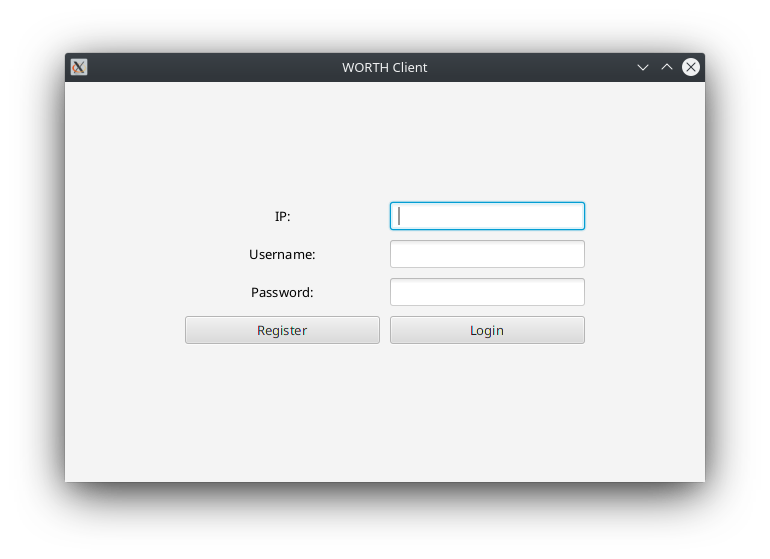
\includegraphics[width=\textwidth]{Login.png}
\end{center}
Una volta inserito l'\code{IP} del server e la combinazione \code{username} e \code{password} si puo' procedere con la registrazione o il login al servizio.
\newpage
Dopo il login ci si trova davanti al menu principale
\begin{center}
    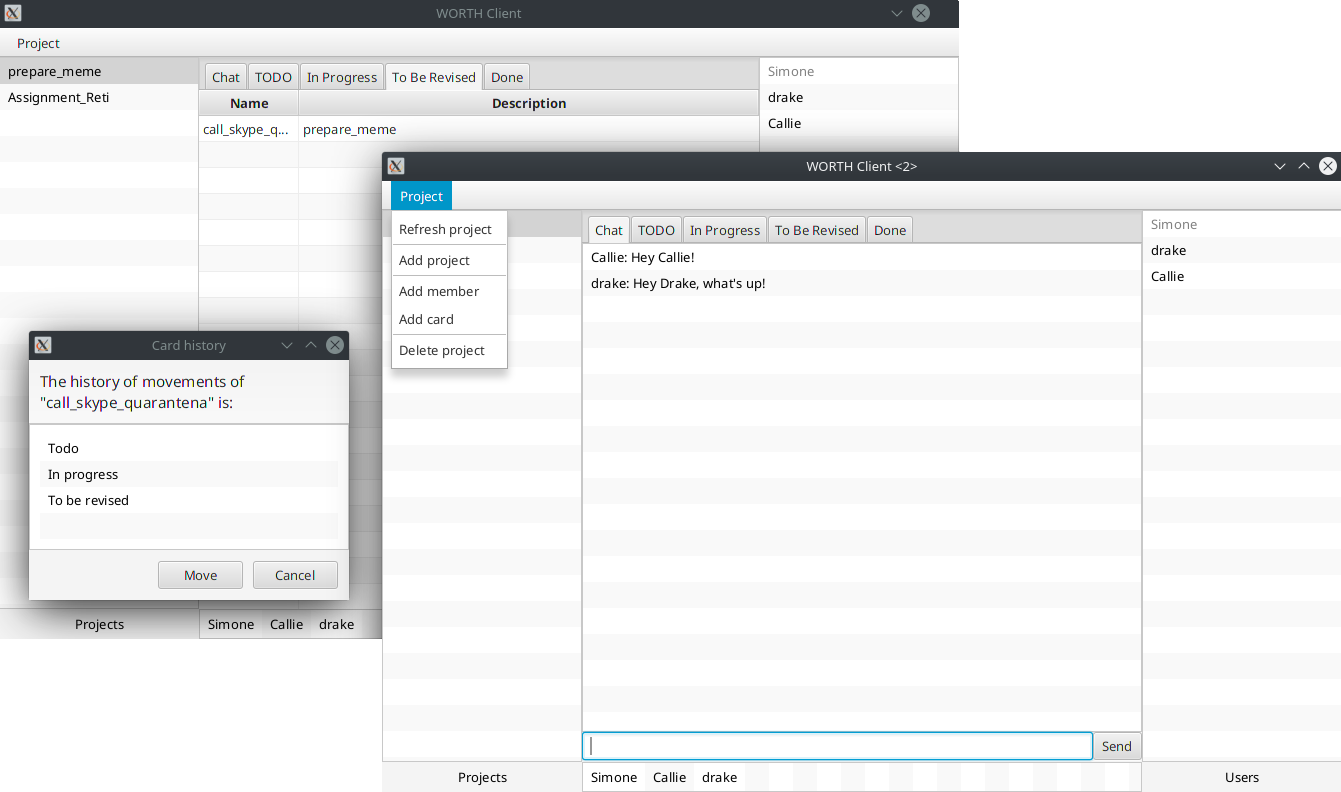
\includegraphics[width=\textwidth]{Main.png}
\end{center}
\paragraph*{La colonna a sinistra} conterrà tutti i progetti di cui l'utente e' membro. Una volta selezionato un progetto e' possibile scrivere sulla chat ed effettuare modifiche su esso.
\paragraph*{La colonna a destra} conterrà tutti i membri del servizio (in {\color{gray}grigio} quelli offline)
\newline
\paragraph*{Il menu in alto} \code{project} contiene i comandi per la creazione e la modifica di un progetto.
\paragraph*{La riga in basso} contiene i nomi dei membri del progetto selezionato.
\paragraph*{La pagina chat} e' utilizzata per visualizzare e inviare messaggi sulla chat del progetto selezionato.
\paragraph*{Le altre pagine} contengono le card dei progetti divise in base al loro stato attuale.
\paragraph*{Selezionando una card} appare lo storico di essa. Da qua, premendo il pulsante \code{Move} e' possibile spostare la card in un'altra lista.
\subparagraph*{Gli spostamenti ammessi sono}
\begin{center}
    \begin{tabular}{||c|c||}
        \hline
        \textbf{Da} & \textbf{Verso}\\
        \hline\hline
        Todo & In Progress\\
        \hline
        In Progress & To Be Revised\\
        \hline
        In Progress & Done\\
        \hline
        To Be Revised & In Progress\\
        \hline
        To Be Revised & Done\\
        \hline
    \end{tabular}
\end{center}